% Template:     Informe LaTeX
% Documento:    Archivo de ejemplo
% Versión:      8.3.6 (23/08/2024)
% Codificación: UTF-8
%
% Autor: Pablo Pizarro R.
%        pablo@ppizarror.com
%
% Manual template: [https://latex.ppizarror.com/informe]
% Licencia MIT:    [https://opensource.org/licenses/MIT]

% ------------------------------------------------------------------------------
% NUEVA SECCIÓN
% ------------------------------------------------------------------------------
% Las secciones se inician con \section, si se quiere una sección sin número se
% pueden usar las funciones \sectionanum (sección sin número) o la función
% \sectionanumnoi para crear el mismo título sin numerar y sin aparecer en el índice
\section{Informes con \LaTeX}

% SUB-SECCIÓN
% Las sub-secciones se inician con \subsection, si se quiere una sub-sección
% sin número se pueden usar las funciones \subsectionanum (nuevo subtítulo sin
% numeración) o la función \subsectionanumnoi para crear el mismo subtítulo sin
% numerar y sin aparecer en el índice
\subsection{Una breve introducción}
	
	Este es un párrafo, puede contener múltiples \quotes{Expresiones} así como fórmulas o referencias\footnote{Las referencias se hacen utilizando la expresión \texttt{\textbackslash label}\{etiqueta\}.} como \eqref{eqn:identidad-imposible} o (\ref{img:anexo-2}). A continuación se muestra un ejemplo de inserción de imágenes (como la Figura \ref{img:testimage}) con el comando \href{https://latex.ppizarror.com/informe.html#hlp-imagen}{\textbackslash insertimage}:

	% Esta instrucción, añadida en la v6.5.5 permite cambiar el título de cada
	% objeto en el índice de cada objeto. Este título es solo válido hasta el
	% primer objeto que lo llame, luego este se restablecerá. Por mientras solo
	% se ofrece compatibilidad para las funciones de imágenes. Los entornos como
	% images o sourcecode aún no tienen compatibilidad
	\setindexcaption{Título de la imagen en el índice.}

	% Para insertar una imagen se puede usar la función \insertimage la cual
	% toma un primer parámetro opcional para definir una etiqueta (dentro de
	% los corchetes), luego toma la dirección de la imagen, sus parámetros
	% (en este caso se definió la escala de 0.12) y una leyenda opcional
	\insertimage[\label{img:testimage}]{ejemplos/test-image.png}{scale=0.12}{Where are you? de \quotes{Internet}.}

	A continuación\footnote{Como se puede observar las funciones \texttt{\textbackslash insert...} añaden un párrafo automáticamente.} se muestra un ejemplo de inserción de ecuaciones simples con el comando \href{https://latex.ppizarror.com/informe.html#hlp-formulae}{\textbackslash insertequation}:

	% Se inserta una ecuación, el primer parámetro entre [] es opcional
	% (permite identificar con una etiqueta para poder referenciarlo después
	% con \ref), seguido de aquello se escribe la ecuación en modo bruto sin signos $
	\insertequation[\label{eqn:identidad-imposible}]{\pow{a}{k}=\pow{b}{k}+\pow{c}{k} \quad \forall k>2}

	% Notar que no se requiere añadir un salto de línea después de insertar una imagen
	Este template \cite{template} ha sido diseñado para que sea completamente compatible con editores \LaTeX\ para escritorio y de manera online\scite{overleaf}. La compilación es realizada siempre usando las últimas versiones de las librerías, además se incluyen los parches oficiales para corregir eventuales \textit{warnings}. \\

	Este es un nuevo párrafo. Para crear uno basta con usar \textbackslash\textbackslash\ en el anterior, lo que fuerza una nueva línea. También se pueden insertar con el comando \texttt{\textbackslash newp} si el compilador de latex arroja una alerta del tipo \textit{Underfull \textbackslash hbox (badness 10000) in paragraph at lines ...}

% SUB-SECCIÓN
\subsection{Añadiendo tablas}

	También puedes usar tablas, ¡Crearlas es muy fácil!. Puedes usar el plugin \href{https://www.ctan.org/tex-archive/support/excel2latex}{Excel2Latex} \cite{excel2latex} de Excel para convertir las tablas a \LaTeX\ o bien utilizar el \quotes{creador de tablas online} \cite{tablesgenerator}.

	% Tabla generada con el plugin Excel2Latex
	\begin{table}[H]
		\centering
		\caption{Ejemplo de tablas.}
		\begin{tabular}{ccc}
			\hline
			\textbf{Columna 1} & \textbf{Columna 2} & \textbf{Columna 3} \bigstrut\\
			\hline
			$\omega$ & $\nu$ & $\delta$ \bigstrut[t]\\
			$\xi$ & $\kappa$ & $\varpi$ \bigstrut[b] \\
			\hline
		\end{tabular}
		\label{tab:tabla-1}
	\end{table}


% ------------------------------------------------------------------------------
% NUEVA SECCIÓN
% ------------------------------------------------------------------------------



\clearpage
\section{Pregunta 2}
\begin{itemize}
	\item \textbf{Escriba las condiciones necesarias para encontrar una solución óptima, utilizando el principio del máximo.}
Se busca el obtener las condiciones necesarias para encontrar la solucion al problema de optimización, utilizando el principio del máximo o Pontryagin. Para ello, se considera el siguiente problema de optimización:
\begin{align}
	 J = \int_{0}^{T} (ph(t) - cu(t))dt
\end{align}
Donde tanto las condiciones de borde como la dinamica del sistema vienen caracterizadas por:
\begin{align}
	\dot{x} = rx(t) \left(1 - \frac{x(t)}{K}\right) - h(t) = 0\\
	x(0) = x_0
\end{align}
Para encontrar la solución óptima, se plantea el Hamiltoniano asociado al problema de optimización:
\begin{align}
	H(x,u,t,\lambda) = ph(t) - cu(t) + \lambda \left( rx(t) \left(1 - \frac{x(t)}{K}\right) - h(t) \right)
\end{align}
Dado que $h(t)=x(t)u(t)$ se reemplaza sobre lo anterior,por lo que el Hamiltoniano se puede reescribir como:
\begin{align}
	H(x,u,t,\lambda) = px(t)u(t) - cu(t) + \lambda \left( rx(t) \left(1 - \frac{x(t)}{K}\right) - x(t)u(t) \right)
\end{align}
Donde los $\lambda$ son los multiplicadores de Lagrange asociados a las restricciones del problema. Luego, se plantean las condiciones de optimalidad asociadas al principio del máximo.
\begin{align}
	\dot{\lambda}&= -\frac{\partial H}{\partial x}\\ 
	             &= -\frac{\partial}{\partial x} \left( px(t)u(t) - cu(t) + \lambda \left( rx(t) \left(1 - \frac{x(t)}{K}\right) - x(t)u(t) \right) \right)\\
				 &= -(pqu(t) + \left(r - \frac{2rx(t)}{K}\right)-qu(t))\lambda) 
\end{align}
Ademas debemos considerar que x(T) es una variable libre dado el enunciado, por lo que tendremos que:
\begin{align}
	\lambda(T) = 0 
\end{align}
Por lo que se obtiene una condicion terminal sobre los multiplicadores. Finalmente para el analisis de la entrada tenemos que considerar que esta puede tomar dos valores, por lo que factorizando el Hamiltoniano en función de u(t) se obtiene que:
\begin{align}
    H = \lambda r x(t) \left( 1 - \frac{x}{K} \right) + u(t) \left( q x(t) (p - \lambda) - c \right)
\end{align}
Vemos por tanto que u(t) es una funcion lineal al hamiltoniano por lo que podemos definir dos condiciones tal que:
\begin{align*}
    u^*(t) &= 0 \quad \text{cuando} \quad q x(t) (p - \lambda(t)) - c < 0 \\
    u^*(t) &= E \quad \text{cuando} \quad q x(t) (p - \lambda(t)) - c > 0
\end{align*}
Por lo que separando por casos se tendra que:
\begin{align}
    \text{Para } u \equiv 0 \text{ tenemos:} \quad
    \begin{cases}
        \dot{x} = r x \left(1 - \frac{x}{K}\right) \\
        \dot{\lambda} = -r \left(1 - \frac{2x}{K}\right) \lambda
    \end{cases}
\end{align}
\begin{align}
    \text{Para } u \equiv E \text{ tenemos:} \quad
    \begin{cases}
        \dot{x} = r x \left(1 - \frac{x}{K}\right) - q x E \\
        \dot{\lambda} = -(p q E + \left(r \left(1 - \frac{2x}{K}\right) - q E\right)\lambda)
    \end{cases}
\end{align}
De esta manera se tiene que el comportamiento de la solución óptima se encuentrara determinada por los diferentes casos de u(t) que se puede caracterizar mediante:
\begin{align}
	F(x,\lambda)= qx(t)(p-\lambda) -c
\end{align}
Donde si es esta es mayor a 0 , se encontrara se tendra que u*(t) = E, mientras que si es menor a 0 se tendra que u*(t) = 0.
	\item \textbf{Simule curvas de nivel en el plano (x, $\phi$), con $\phi$ el coestado. Interprete los resultados y concluya sobre el comportamiento óptimo de u(t).}\\
Se busca obtener las curvas de nivel en el plano (x, $\lambda$) para esto se hace uso de \textit{Matlab} y en particular la funcion \textit{ODE45} tal que permita resolver las ecuaciones diferenciales asociadas a las condiciones de optimalidad obtenidas en el punto anterior para los diferentes casos, dando como resultado lo siguiente:
\begin{figure}[H]
	\centering
	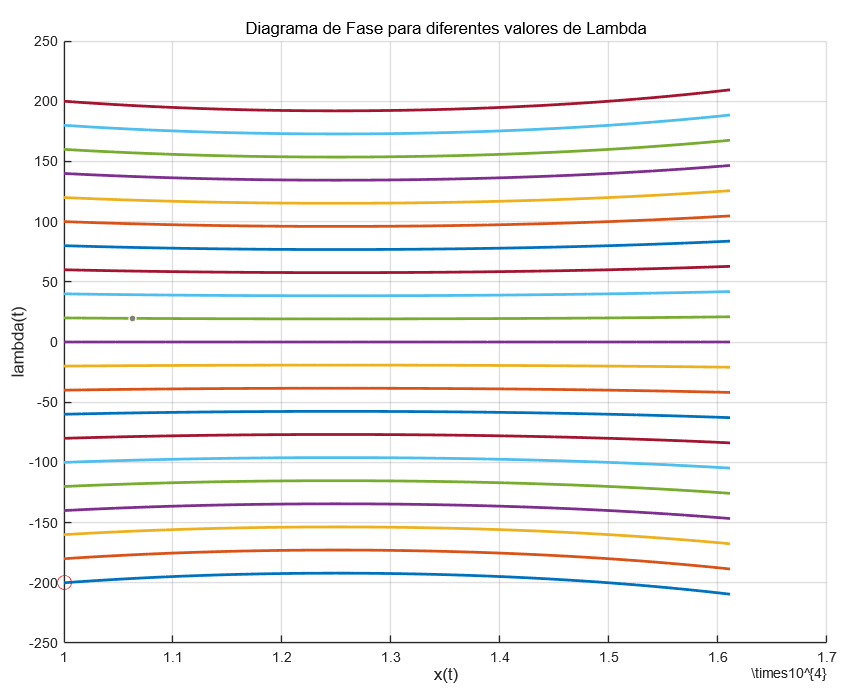
\includegraphics[width=0.6\textwidth]{img/Grafico u=0.png}
	\caption{Curvas de nivel en el plano (x, $\lambda$) tanto para $u=0$ para los diferentes valores de $\lambda_{0}$, en un rango de de -200 -- 200}
	\label{img:curvas-nivel}
\end{figure}
Por otro lado tenemos que:
\begin{figure}[H]
	\centering
	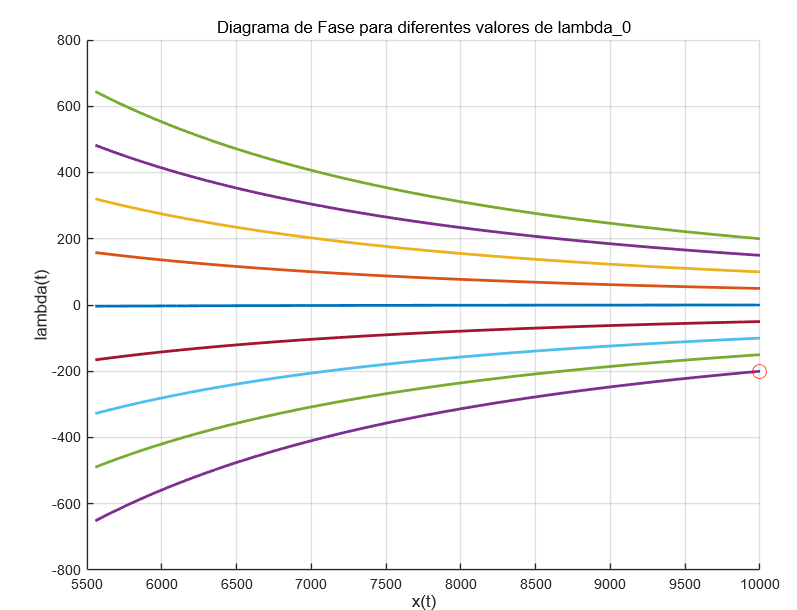
\includegraphics[width=0.6\textwidth]{img/Grafico u=E.png}
	\caption{Curvas de nivel en el plano (x, $\lambda$) para $u=E$ para los diferentes valores de $\lambda_{0}$, en un rango de de -200 -- 200.}
	\label{img:curvas-nivel}
\end{figure}
Luego se puede observar que el comportamiento de la solución óptima se encuentra determinada por los diferentes casos de u(t), ademas de el valor de la condicion inicial $\lambda_0$.
	\item \textbf{Encuentre una expresión para la acción de control óptima $u^{∗}(t)$ y la dinámica de la
	población de peces resultante $x^{*}(t)$, en función de las constantes conocidas. Grafique e interprete los
	resultados.}\\\\
Dado que se busca encontrar una expresion para la acción de control óptima $u^{∗}(t)$ y la dinámica de la población de peces resultante $x^{*}(t)$, en función de las constantes conocidas, se tiene que la acción de control óptima se encuentra determinada por los diferentes casos de u(t), donde para un cierto $t_{c}$ se tendra que usaremos $u=0$ y para $t>t_{c}$ se tendra que $u=E$, pero es importante notar que el comportamiento esta fuertemente determinado por la condicion inicial ($\lambda_{0})$ y que ademas se debe cumplir que
\begin{align}
	\lambda(T)=0 
\end{align}
Por lo que analizando las curvas de nivel anteriores, se tendra que para que dicha condicion terminal se cumpla se debe tener que en todo momento $u(t)=E$. Es por esto que nos quedaremos con esta solución, por lo que se tiene que:
\begin{align}
    \text{Para } u \equiv E \text{ tenemos:} \quad
    \begin{cases}
        \dot{x} = r x \left(1 - \frac{x}{K}\right) - q x E \\
        \dot{\lambda} = -(p q E + \left(r \left(1 - \frac{2x}{K}\right) - q E\right)\lambda)
    \end{cases}
\end{align}
Luego se deberan resolver estas ecuaciones, dando como resultado:
\begin{align}
	\dot{x} & = r x \left(1 - \frac{x}{K}\right) - q x E \\
	        &= rx - \frac{r}{k}x^{2} - qxE\\
			&= -\frac{r}{k}x^{2} + x(r-qE)
\end{align}
Si reemplazamos los valores de r,q y E. Se obtiene que (r-qE) = 0, por lo que se tiene que:
\begin{align}
	\dot{x} = -\frac{r}{k}x^{2}
\end{align}
Resolviendo la ecuacion diferencial se tiene que:
\begin{align}
	x(t) = \frac{1}{\frac{r}{K}t - C}
\end{align}
Luego como conocemos x(0)= $x_0$, se tiene que:
\begin{align}
	x(0) = \frac{1}{\frac{r}{K} \cdot 0 - C} = -\frac{1}{C}
\end{align}
Con lo que tenemos finalmente que:
\begin{align}
	x(t) = \frac{1}{\frac{r}{K}t + \frac{1}{x_0}}
\end{align}
Esto por lo mencionado anteriormente es valido para $t \in \left[ 0,T\right]$, luego tenemos que para $\lambda$ viene dado por:
\begin{align}
	\dot{\lambda} &= -(p q E + \left(r \left(1 - \frac{2x}{K}\right) - q E\right)\lambda)\\
	& = - (pqE + \frac{2r}{K}x \lambda)
\end{align}
Dado que nos piden el obtener la dinámica de la población de peces resultante $x^{*}(t)$, se obtiene el siguiente grafico:
\begin{figure}[H]
	\centering
	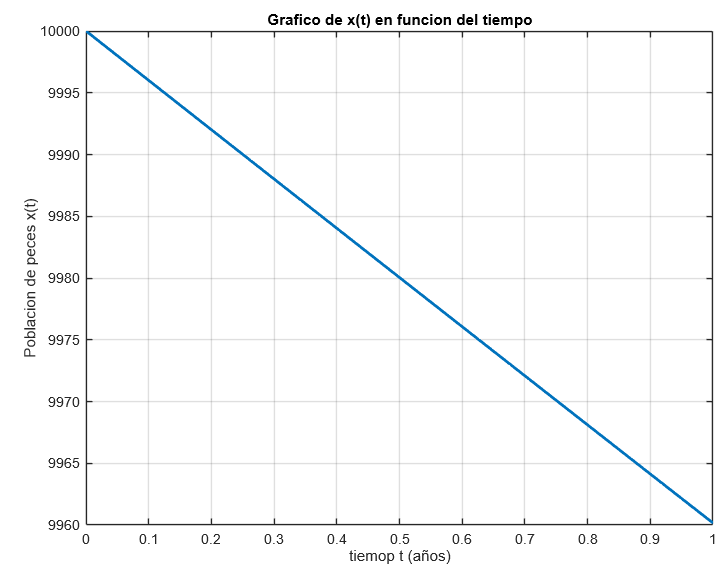
\includegraphics[width=0.6\textwidth]{img/[P2] Grafico de x(t).png}
	\caption{Grafico de x(t) que representa el número de peces en el lago en función del tiempo.}
	\label{img:curvas-nivel}
\end{figure}
Luego tenemos que la entrada óptima $u^{*}(t)$ se encuentra dada por:
\begin{figure}[H]
	\centering
	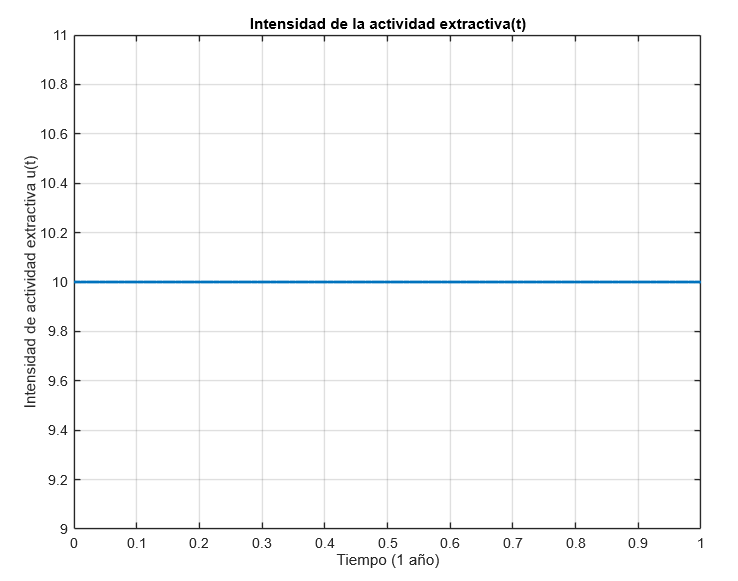
\includegraphics[width=0.6\textwidth]{img/[P2] Grafico de u(t).png}
	\caption{Grafico de u(t)=E optimo,  que representa la actividad pesquera (medida en cantidad de botes pesqueros en el lago).}
	\label{img:curvas-nivel}
\end{figure}
\item \textbf{Encuentre el valor óptimo de J. Evalúe J para otra acción de control (no óptima) y
concluya}\\\\
Retomando la funcion de costos dada por:
\begin{align}
	J(x(t),u(t))= \int_{0}^{T} (ph(t) - cu(t))dt
\end{align}
Luego tenemos que el valor óptimo de J evaluado en los valores optimos de x(t) y u(t) se tiene que:
\begin{align}
	J(x^{*}(t),u^{*}(t))&= \int_{0}^{T} (ph(t) - cu(t))dt\\
	&= \int_{0}^{1} (pqx(t)u(t) - cu(t))dt\\
	&= \int_{0}^{1} (1\cdot 10^{-3} \cdot 10 \cdot \frac{1}{\frac{0.01}{25.000}t + \frac{1}{10000}} - 10)dt\\
	&= 89.8005
\end{align}
Con lo que se maximiza el valor de J, por otro lado si se evalua J para una acción de control no optima por ejemplo con un u(t) = 5 , se tiene que:
\begin{align}
	J(x^{*}(t),u^{*}(t))&= \int_{0}^{T} (ph(t) - cu(t))dt\\
	&= \int_{0}^{1} (pqx(t)u(t) - cu(t))dt\\
	&= \int_{0}^{1} (1\cdot 10^{-3} \cdot 5 \cdot \frac{1}{\frac{0.01}{25.000}t + \frac{1}{10000}} - 5)dt\\
	&= 44.9003
\end{align}
Por lo que se tiene que el valor de J es menor que el valor optimo, por lo que se concluye que la acción de control optima es la que maximiza el valor de J.
\end{itemize}
\section{Pregunta 3}
\begin{itemize}
	\item \textbf{Represente el sistema en variables de estado, indicando las matrices/vectores de estado A, B, C, y D. ¿Qué representan dichas matrices? Además, estudie la controlabilidad observabilidad y estabilidad del sistema.}\\\\
	Luego se busca el representar el sistema en variables de estado, por lo que se debe considerar la siguiente ecuación diferencial:
	\begin{align}
		\dot{\alpha}(t) &= -0.3130\alpha(t) + \dot{\theta}(t) + 0.2320\delta(t) \\
		\dot{q}(t) &= -0.0139\alpha(t) - 0.4260q(t) + 0.0203\delta(t) \\
		\dot{\theta}(t) &= 56.70q(t)
	\end{align}
	Donde podemos definir las variables de estado como:
	\begin{align}
		x_1(t) &= \alpha(t) \\
		x_2(t) &= q(t) \\
		x_3(t) &= \theta(t)
	\end{align}
	Donde se tendra que la variable de control o manipulada sera $\delta(t)$, por lo que se tiene que:
	\begin{align}
		\dot{x}(t) &= A x(t) + B u(t) \\
		y(t) &= C x(t) 
		\end{align}
		
		Donde:
		\[
		x(t) = \begin{bmatrix}
			x_1(t) \\
			x_2(t) \\
			x_3(t)
		\end{bmatrix}, \quad u(t) = \delta(t), \quad y(t) = \theta(t)
		\]
		
		Las matrices $A$, $B$, $C$ y $D$ son las siguientes:
		
		\begin{align}
		A &= \begin{bmatrix}
			-0.3130 & 56.70 & 0 \\
			-0.0139 & -0.4260 & 0 \\
			0 & 56.70 & 0
		\end{bmatrix}, \\
		B &= \begin{bmatrix}
			0.2320 \\
			0.0203 \\
			0
		\end{bmatrix}, \\
		C &= \begin{bmatrix}
			0 & 0 & 1
		\end{bmatrix}, \\
		D &= \begin{bmatrix}
			0
		\end{bmatrix}
		\end{align}		
Donde se tiene que la variable de salida o controlada corresponde a el angulo de inclinacion $\theta(t)$ por esa razon C, tiene la forma previamente mencionada. Esta matrices se puede interpretar como:
\begin{itemize}
	\item \textbf{Matriz A}: Representa la dinamica del sistema, es decir, como evolucionan las variables de estado en el tiempo, permite ademas se relaciona de manera directa con la matriz de transicion de estados y nos permite tener un conocimiento en cuanto a la estabilidad del sistema.
	\item \textbf{Matriz B}: Representa la influencia de la variable de control sobre las variables de estado, es decir, como la variable de control afecta a las variables de estado.
	\item \textbf{Matriz C}: Representa la influencia de las variables de estado sobre la variable de salida, es decir, como las variables de estado afectan a la variable de salida, basicamente nos da la libertad para analizar que variables son de interes en el analisis.
	\item \textbf{Matriz D}: Representa la influencia de la variable de control sobre la variable de salida, usualmente se considera 0 dado que es simplemente un \textit{Outset} de la variable de control.
\end{itemize}
Buscamos analizar controlabilidad de nuestro sistema, es por esto que se utiliza la matriz: 
\begin{align}
	\mathcal{C} = \begin{pmatrix} B & AB & A^{2}B & \dots & A^{n-1}B \end{pmatrix}
\end{align}
Dado que en nuesto caso particular n=3,se tiene que:
\begin{align}
	\mathcal{C} = \begin{pmatrix} B & AB & A^{2}B\end{pmatrix}
\end{align}
Dado los valores de A y B previamente obtenidos, luego tenemos que la matriz de controlabilidad sera:
\begin{align}
	C = \begin{bmatrix}
		0.232 & 1.0784 & -1.0107 \\
		0.0203 & -0.0119 & -0.0099 \\
		0 & 1.1510 & -0.6732
	\end{bmatrix}
	\end{align}
Luego se observa que tanto filas como columnas son LI por lo que el sistema es controlable, dado que es de rango completo.Por otro lado se busca analizar la observabilidad del sistema, es por esto que se utiliza la matriz:
\begin{align}
	\vartheta = \begin{pmatrix} C \\ CA \\ CA^{2} \\ \vdots \\ CA^{n-1} \end{pmatrix}
\end{align}
Luego para nuestro caso particular se tiene que:
\begin{align}
	\vartheta = \begin{pmatrix} C \\ CA \\ CA^{2} \end{pmatrix}
\end{align}
Al ser calculada se tiene que:
\begin{align}
	\vartheta = \begin{bmatrix}
		0 & 0 & 1 \\
		0 & 56.70 & 0 \\
		-0.7881 & -24.1542 & 0
	\end{bmatrix}
\end{align}
Al igual que antes vemos que el sistema es de rango completo y que tanto sus filas como columnas son LI, por lo que el sistema es observable. Finalmente se busca analizar la estabilidad del sistema, es por esto que se busca analizar los valores propios de la matriz A, dado que estos determinan la estabilidad del sistema, se tiene que:
\begin{align}
	\text{det}(A - \lambda I) = 0
\end{align}
Luego mediante Matlab , se tiene que los valores propios vienen dados por:
\begin{align}
	\lambda_{1} &= 0\\
	\lambda_{2} &= −0.3695+0.88596713j\\
	\lambda_{3} &= −0.3695-0.88596713j
\end{align}
Se observa por tanto que el sistema es criticamente estable, dado que tiene un polo en 0

	\item  \textbf{Obtenga la función de transferencia y diseñe un controlador PI que cumpla con los criterios de diseño mencionados anteriormente (en caso de no lograr cumplir con los requerimientos, mencione cuales si se logran cumplir). Simule y grafique la variable manipulada y controlada. Sea específico/a con el método de sintonización utilizado}\\\\
	Para obtener la función de transferencia se utiliza la funcion ss2tf de Matlab, la cual permite obtener la función de transferencia a partir de las matrices A,B,C y D, luego se obtiene que:
	\begin{align}
		\frac{Y(s)}{U(s)} = \frac{1.151s+0.1774}{s^{3} + 0.739s^{2} + 0.9215s}
	\end{align}
	Luego se propone un PI, el cual tiene ls siguiente forma:
	\begin{align}
		G_{c}(s) = K_{p} + \frac{K_{i}}{s}
	\end{align}
	Mediante la herramienta de \textit{PID Tool} de Matlab, se obtiene que los valores de $K_{p}$ y $K_{i}$ optimos son:
	\begin{align}
		K_{p} &= 0.24289\\
		K_{i} &= 0.31544
	\end{align}
	Se tiene que el sistema bajo este controlador tiene el siguiente desempeño:
	\begin{table}[h!]
		\centering
		\begin{tabular}{|c|c|}
		\hline
		\textbf{Valores de desempeño} & \textbf{Valores} \\
		\hline
		Rise time & 1.97 seconds \\
		\hline
		Settling time & 19.3 seconds \\
		\hline
		Overshoot & 22.1\% \\
		\hline
		Peak & 1.22 \\
		\hline
		\end{tabular}
		\caption{Valores de desempeño obtenidos luego de optimizar los valores del controlador PI}
		\end{table}
	Se observa que cumple con los requerimientos asocados al \textit{Rise time}, al \textit{Settling time} y al cero error a estado estacionario, pero no cumple con el requerimiento de overshoot, dado que este es mayor al 20\%, se realizaron variados intentos y no se logra cumplir con este requerimiento del \textit{Overshoot} y \textit{Settling time}, en simultaneo.Luego se obtienen las siguientes respuestas del sistema:
	\begin{figure}[H]
		\centering
		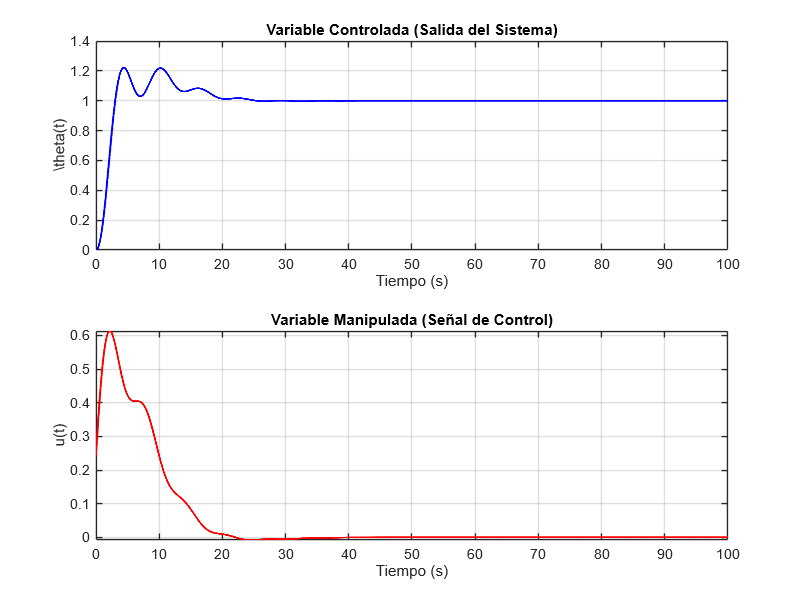
\includegraphics[width=0.8\textwidth]{img/[P3]Respuesta al escalon.png}
		\caption{Repuesta manipulada y respuesta al escalon del sistema .}
		\label{img:curvas-nivel}
	\end{figure}
	Se obtiene finalmente los graficos de interes, asi como la sintonización para el controlador PI

\end{itemize}
%-------------------	-----------------------------------------------------------
% SUB-SECCIÓN
% ------------------------------------------------------------------------------
